\section{Factory}
\begin{figure}[H]
    \centering
    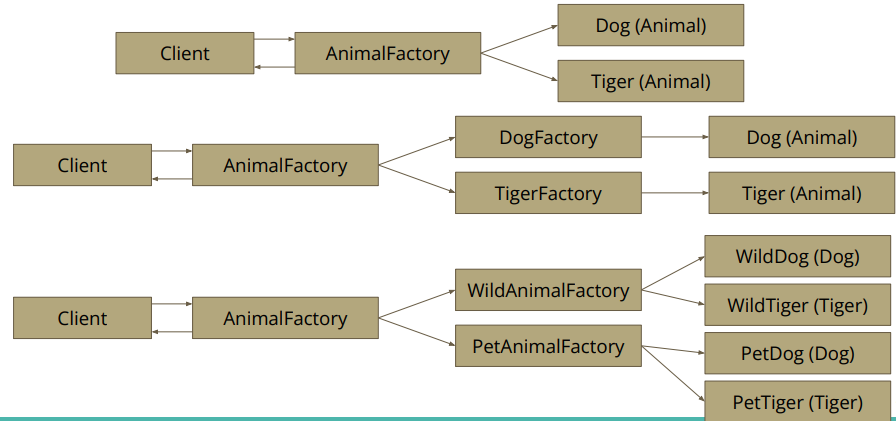
\includegraphics[width=\linewidth]{chapters/design_patterns/figures/factory_pattern_base.png}
\end{figure}
\clearpage
\subsection{Simple Factory}
\begin{lstlisting}
class AnimalFactory {
    public Animal createAnimal(Type animalType) {
        Animal animal = null;
        if (animalType.equals(Type.DOG)) {
            animal = new Dog();
        } else if (animalType.equals(Type.TIGER)) {
            animal = new Tiger();
        } else if (animalType.equals(Type.CAT)) {
            animal = new Cat();
        }
        return animal;
    }
}
         
\end{lstlisting}

\clearpage
\subsection{Factory Pattern}
An object with a method that creates new objects using abstraction.
\begin{lstlisting}
// Base factory
abstract class AnimalFactory {
    public abstract Animal createAnimal();
}

// One factory using the base factory
class DogFactory extends AnimalFactory {
    public Animal createAnimal() {
        return new Dog();
    }
}

// Usage of factory
AnimalFactory factory = new DogFactory();
Animal animal = factory.createAnimal();
animal.displayBehavior();
\end{lstlisting}

\clearpage
\subsection{Abstract Factory}
\begin{lstlisting}
// Base factory
interface AnimalFactory {
    Tiger createTiger();
    Dog createDog();
}

// Wild factory
public class WildAnimalFactory implements AnimalFactory {
    public Tiger createTiger() { ... }
    public Dog createDog() { ... }
}

// Pet factory
public class PetAnimalFactory implements AnimalFactory {
    public Tiger createTiger() { ... }
    public Dog createDog() { ... }
}

// Usage
AnimalFactory factory = new WildAnimalFactory();
Animal animal = factory.createTiger();
animal.displayBehavior();
\end{lstlisting}